\documentclass[12pt,a4paper]{article}

\usepackage[T1]{fontenc}
\usepackage[utf8]{inputenc}
\usepackage[brazilian]{babel}
\usepackage{newtxtext,newtxmath}
\usepackage{amsmath}
\usepackage{graphicx}
\usepackage{booktabs}
\usepackage{geometry}
\usepackage{setspace}
\usepackage{indentfirst}
\usepackage{float}
\usepackage{caption}
\usepackage{subcaption}
\usepackage{hyperref}
\usepackage{placeins}

\geometry{margin=2.6cm}
\onehalfspacing
\setlength{\parindent}{1.25cm}
\setlength{\parskip}{0pt}
\graphicspath{{report_assets/}}

\begin{document}
\pagenumbering{gobble}

\begin{titlepage}
    \centering
    {\Large \textbf{CENTRO FEDERAL DE EDUCAÇÃO TECNOLÓGICA CELSO\\SUCKOW DA FONSECA}\par}
    \vspace{0.25cm}
    {\Large CAMPUS MARACANÃ\par}
    {\Large ENGENHARIA ELETRÔNICA\par}
    {\Large PROCESSAMENTO DE SINAIS I\par}

    \vfill

    {\LARGE \textbf{RELATÓRIO DA PRÁTICA 7: PROJETO DE\\FILTROS FIR}\par}

    \vfill

    {\large
    Pedro Nicollas Pereira Azevedo Della Torre Bastos\par
    Gabriel Florencio da Fonseca\par
    Ricardo Alexandre Vieira da Silva\par}

    \vfill

    {\large Rio de Janeiro, Brasil\par}
    {\large Junho de 2026\par}
\end{titlepage}

\clearpage
\pagenumbering{arabic}
\setcounter{page}{1}

\section*{Objetivos}
Esta prática teve como objetivo projetar e analisar filtros digitais FIR sem utilizar funções prontas de projeto. O foco principal foi o método de janelamento aplicado a respostas ao impulso ideais, investigando como a ordem do filtro e a janela escolhida afetam largura de transição, ripples, seletividade e distribuição de zeros.

Também foram estudadas três respostas ideais não triviais, derivadas diretamente a partir de módulos especificados no domínio da frequência. Por fim, o projeto foi aplicado à recuperação do arquivo de áudio \texttt{handel.wav}, com comparação explícita em relação à solução IIR usada na Prática 6 e avaliação do efeito da quantização dos coeficientes.

\section*{Materiais Utilizados}
Foram utilizados Python 3.11, NumPy, SciPy, Matplotlib e notebooks Jupyter para o cálculo dos coeficientes, geração de respostas em frequência, diagramas de polos e zeros, métricas numéricas e simulações com áudio. O arquivo \texttt{handel.wav}, localizado na pasta \texttt{data}, foi utilizado na etapa de filtragem.

O projeto FIR foi implementado diretamente a partir das expressões analíticas das respostas ideais. Para um filtro passa-baixas com frequência de corte $\omega_c$, foi usada a forma centrada
\[
h_{PB}[n] =
\begin{cases}
\dfrac{\omega_c}{\pi}, & n = 0,\\[4pt]
\dfrac{\sin(\omega_c n)}{\pi n}, & n \neq 0.
\end{cases}
\]
As demais respostas foram obtidas por combinação dessa base:
\[
h_{PA}[n] = \delta[n] - h_{PB}[n], \qquad
h_{PF}[n] = h_{PB,2}[n] - h_{PB,1}[n], \qquad
h_{RF}[n] = \delta[n] - h_{PF}[n].
\]

Em todos os casos, o filtro causal final foi construído por truncamento em $M+1$ amostras seguido da multiplicação por uma janela $w[n]$, isto é,
\[
h[n] = h_d[n - M/2]\,w[n].
\]

\section*{Metodologia}
A metodologia foi organizada em três blocos. Na primeira etapa, foram projetados filtros passa-baixas, passa-altas, passa-faixas e rejeita-faixas para $f_s = 20000$ Hz, usando ordens $M \in \{20, 50, 100\}$ e as janelas retangular, triangular, Bartlett, Hamming, Hann e Blackman.

Na segunda etapa, foram derivadas as respostas ao impulso ideais correspondentes às três formas de módulo apresentadas no enunciado. Para o item 2(b), a expressão permaneceu simbólica na dedução, mas os gráficos numéricos adotaram $\omega_c = \pi/8$, de forma que o suporte da resposta triangular ficasse em $[-\pi/4, \pi/4]$.

Na terceira etapa, foi construído um sistema de filtragem FIR para o áudio contaminado:
\[
y(t) = x(t) + 0.05\cos(200\pi t) + 0.075\sin(4000\pi t) + n(t).
\]
O sistema escolhido foi uma cascata linear de fase composta por:
\begin{itemize}
    \item passa-altas FIR Blackman com $f_c = 180$ Hz e ordem $M = 120$;
    \item rejeita-faixas FIR Blackman de 1850 Hz a 2150 Hz e ordem $M = 260$;
    \item passa-baixas FIR Blackman com $f_c = 2400$ Hz e ordem $M = 100$.
\end{itemize}
O atraso total do sistema foi de 240 amostras, equivalente a aproximadamente 29,3 ms, compensado nas métricas e comparações temporais.

\section*{Questão 1: Projeto FIR por Janelamento}
Na primeira questão, foram projetados quatro tipos de filtros FIR com especificações diretas em frequência: passa-baixas em 1000 Hz, passa-altas em 2000 Hz, passa-faixas de 500 Hz a 2000 Hz e rejeita-faixas de 1000 Hz a 2500 Hz. Para facilitar a leitura do relatório, a Figura~\ref{fig:q1-respostas} fixa a ordem em $M=100$ e compara apenas o efeito das janelas; os notebooks contêm as famílias completas para todas as ordens.

\begin{figure}[H]
    \centering
    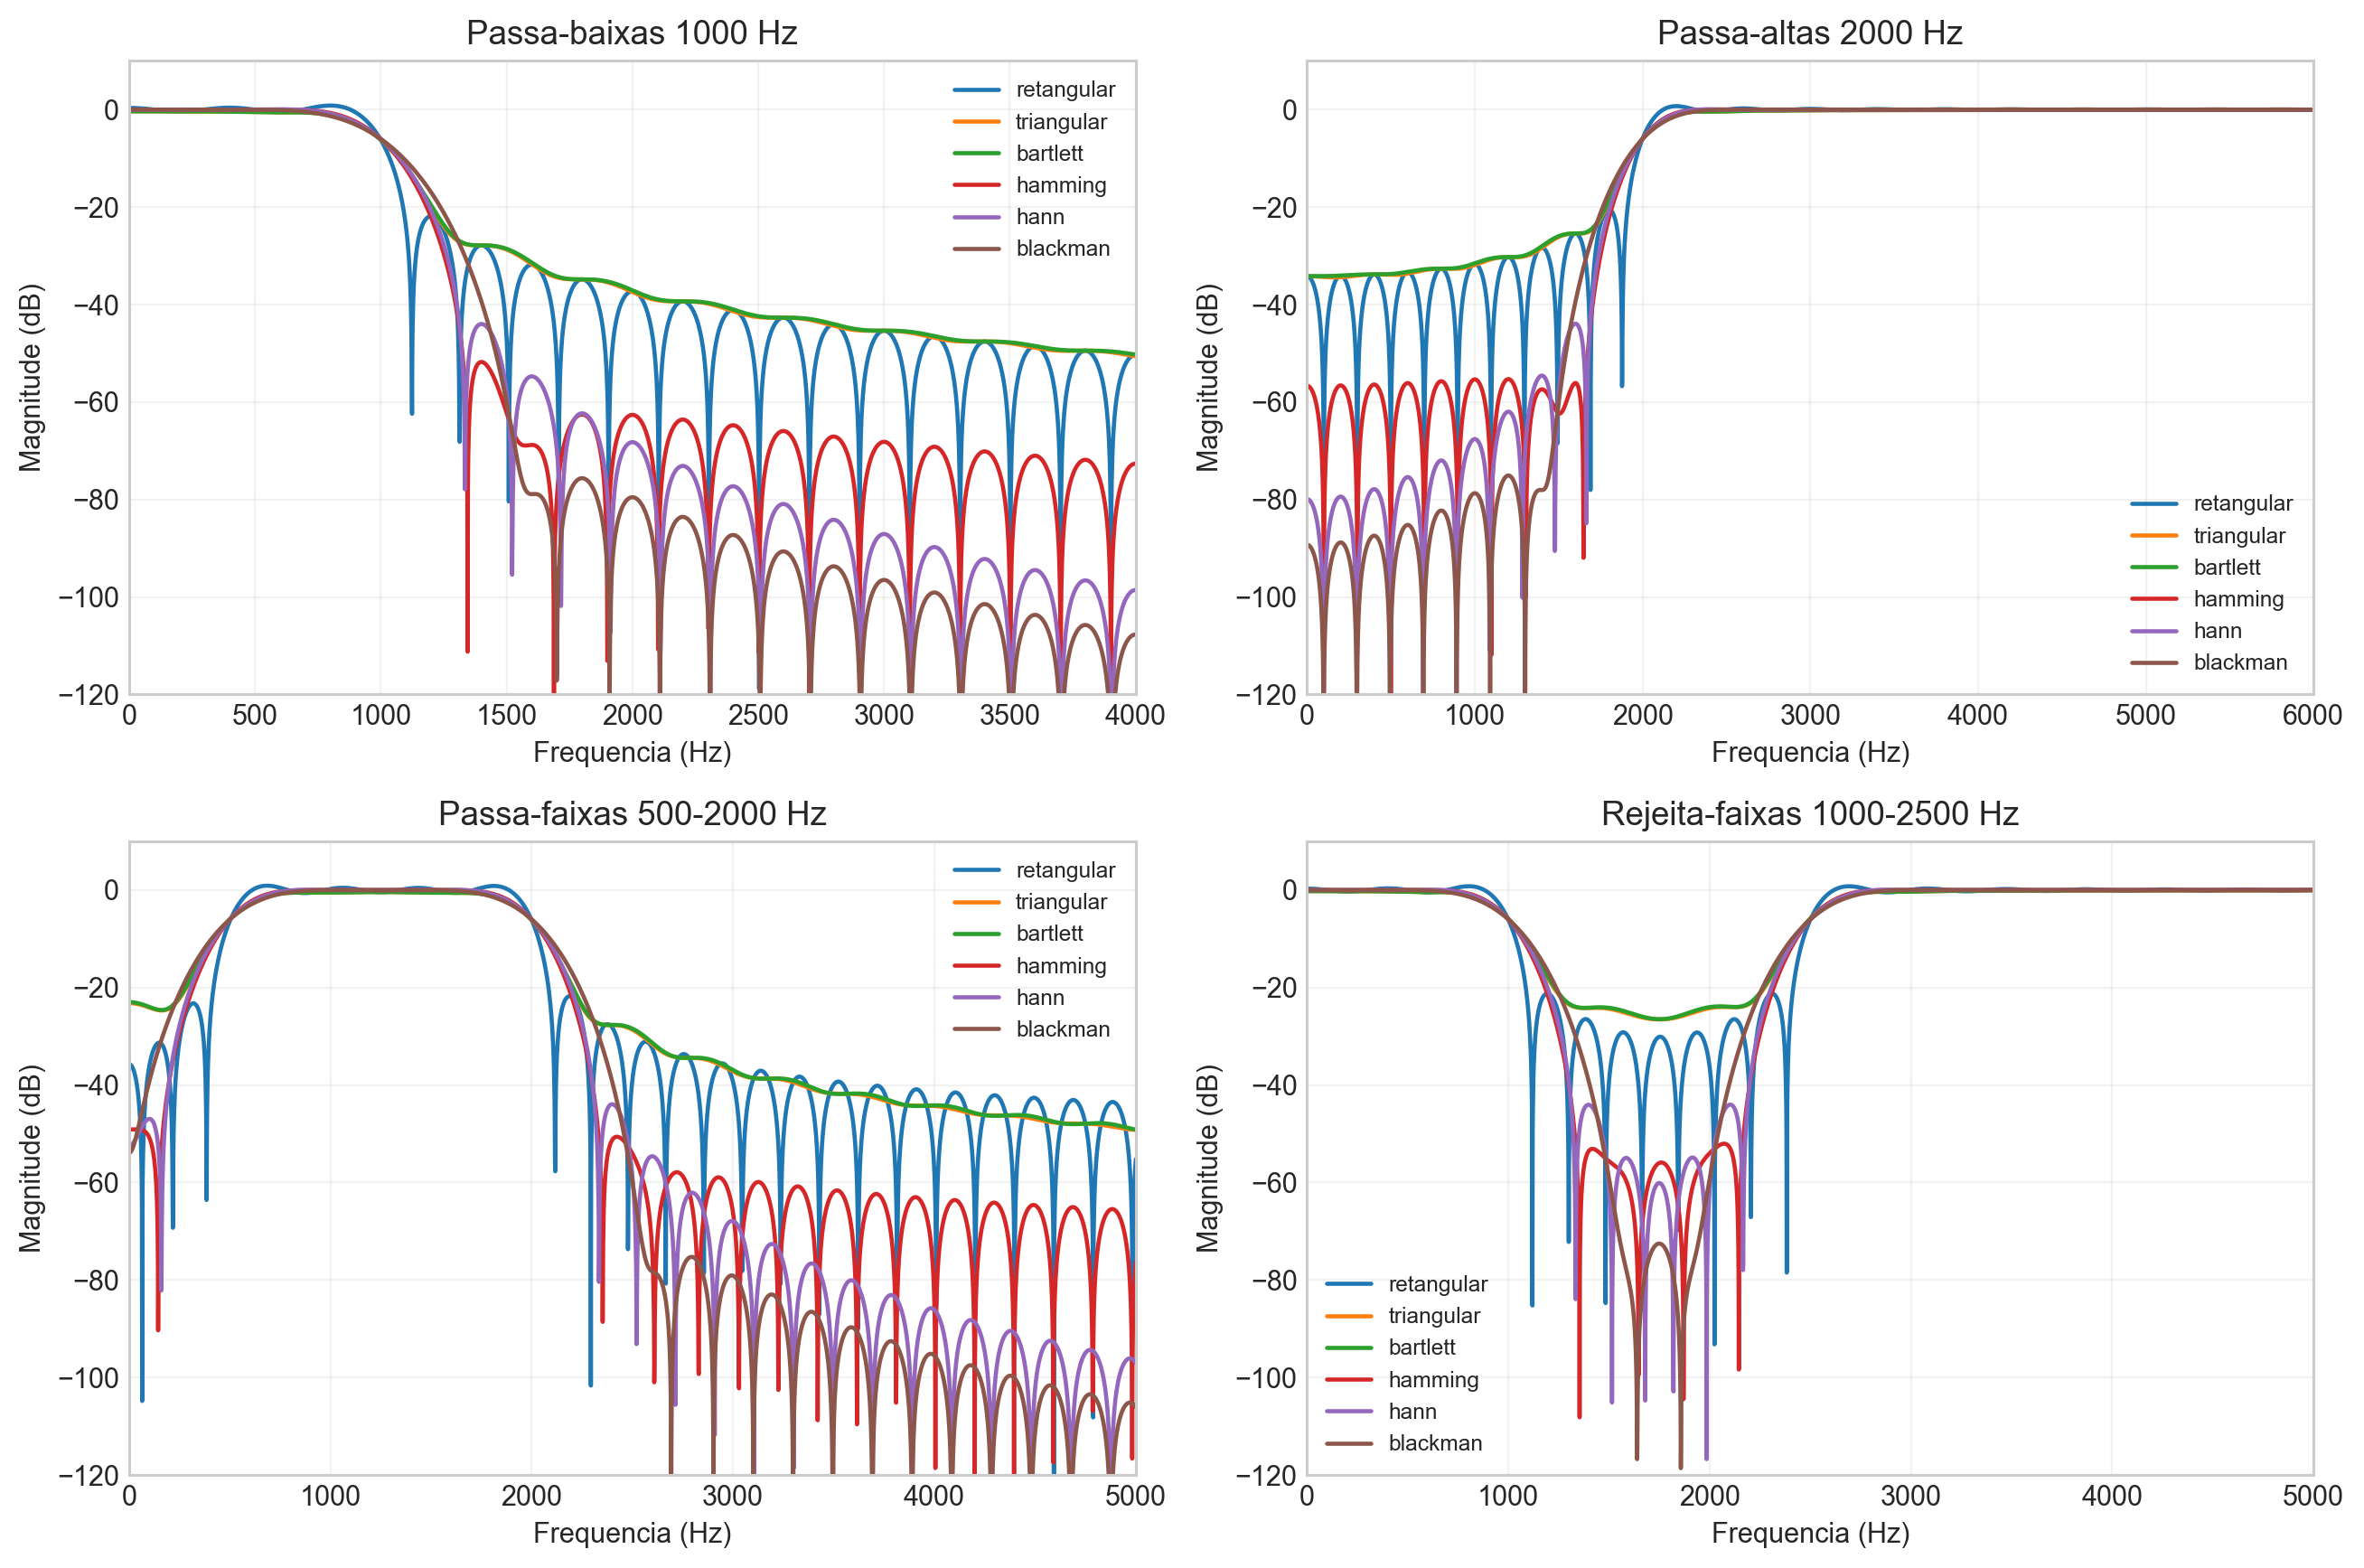
\includegraphics[width=\textwidth]{q1_responses_m100.png}
    \caption{Respostas em frequência dos filtros da Questão 1 para $M=100$ e diferentes janelas.}
    \label{fig:q1-respostas}
\end{figure}

\begin{figure}[H]
    \centering
    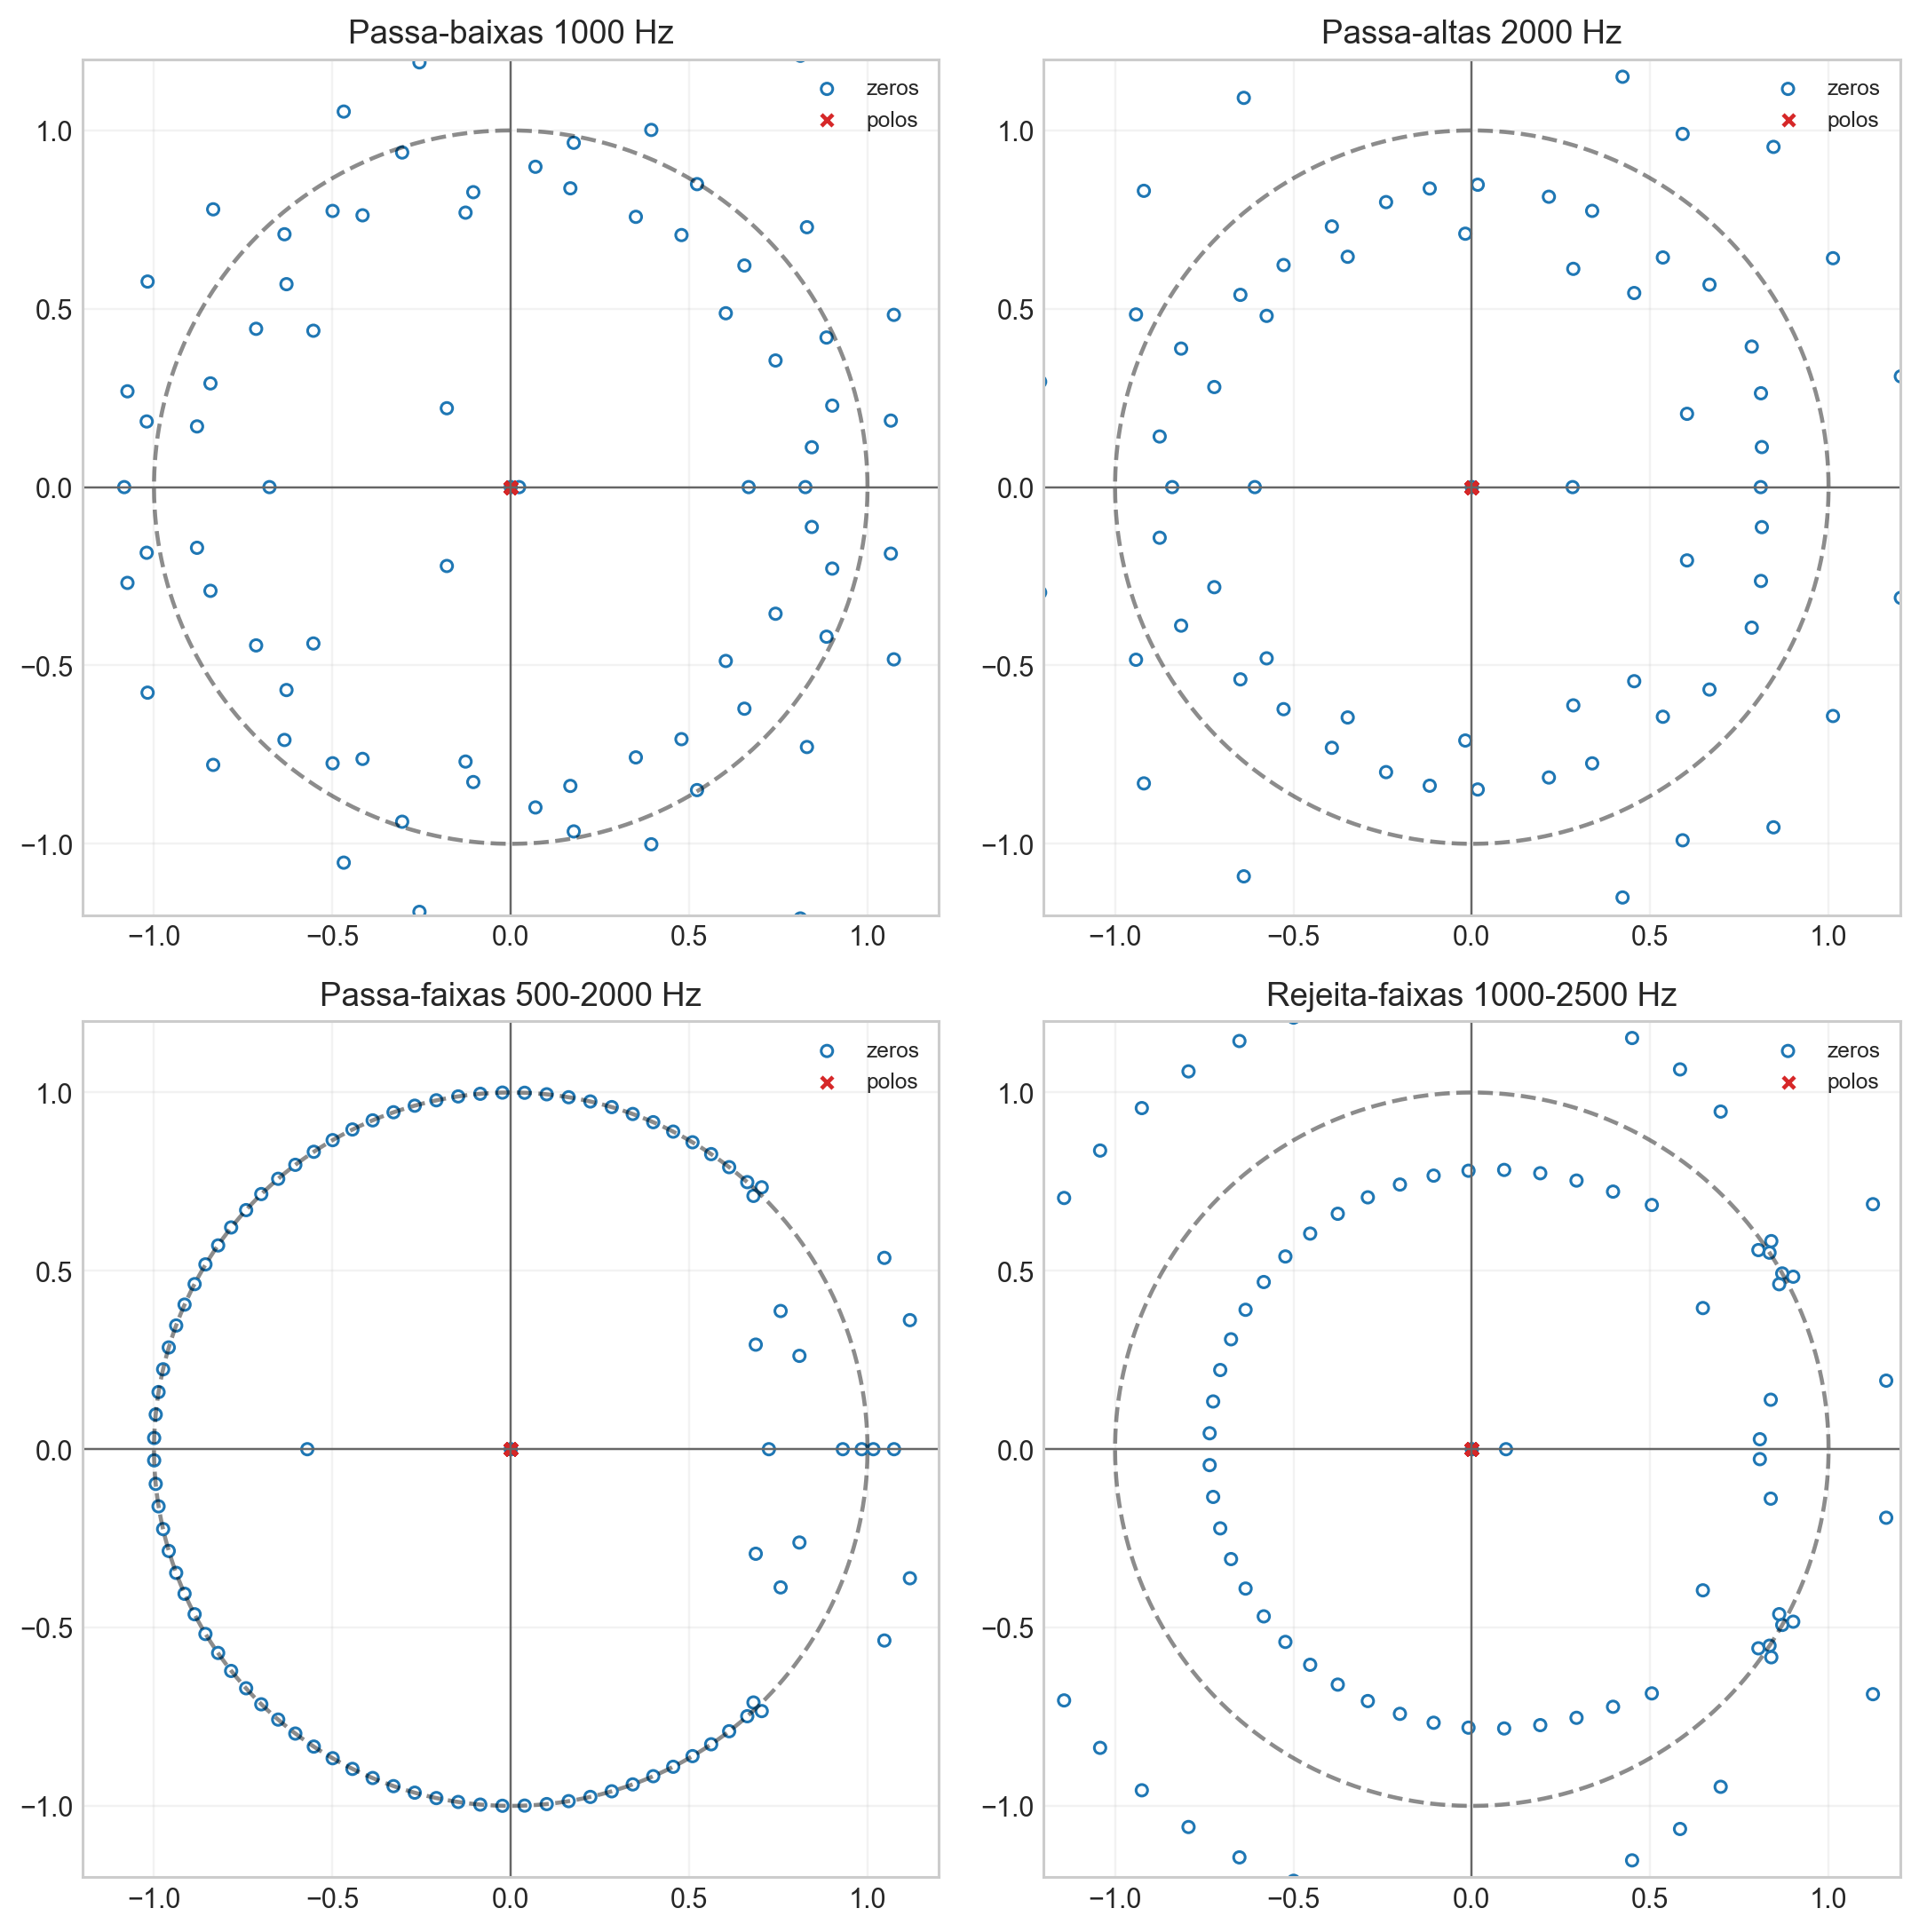
\includegraphics[width=0.9\textwidth]{q1_pz_blackman_m100.png}
    \caption{Diagramas de polos e zeros representativos da Questão 1 usando janela Blackman e $M=100$.}
    \label{fig:q1-pz}
\end{figure}

\begin{table}[H]
    \centering
    \caption{Erro RMS global da aproximação usando janela Blackman para diferentes ordens.}
    \begin{tabular}{lccc}
\toprule
Filtro & $M=20$ & $M=50$ & $M=100$ \\
\midrule
Passa-baixas 1000 Hz & 0,1567 & 0,0936 & 0,0662 \\
Passa-altas 2000 Hz & 0,1481 & 0,0936 & 0,0662 \\
Passa-faixas 500-2000 Hz & 0,2334 & 0,1341 & 0,0936 \\
Rejeita-faixas 1000-2500 Hz & 0,2348 & 0,1325 & 0,0936 \\
\bottomrule
\end{tabular}
\end{table}

Os resultados mostram o efeito esperado do aumento de ordem: os erros caem sistematicamente de $M=20$ para $M=100$, principalmente nos casos passa-faixas e rejeita-faixas, que exigem transições duplas. Visualmente, a janela retangular oferece a transição mais estreita, mas exibe os maiores lobos secundários. Já Hamming, Hann e Blackman reduzem ripples fora da banda às custas de transições mais largas.

Como todo filtro FIR causal possui denominador unitário, todos os polos ficam concentrados na origem. Assim, o projeto é sempre BIBO estável, e a diferença entre as alternativas aparece principalmente no posicionamento dos zeros próximos ao círculo unitário e na forma da resposta em frequência. Isso torna os diagramas de polos e zeros menos dramáticos do que na prática de IIR, mas ainda úteis para visualizar as frequências rejeitadas.

\section*{Questão 2: Respostas Ideais Derivadas}
Na segunda questão, foi necessário partir da forma do módulo e derivar a resposta ao impulso ideal correspondente. Para o item (a), a resposta em frequência equivale à soma de dois passa-baixas ideais:
\[
H_a(\omega) =
\begin{cases}
2, & |\omega| \le \pi/6,\\
1, & \pi/6 < |\omega| \le \pi/3,\\
0, & \pi/3 < |\omega| \le \pi.
\end{cases}
\]
Da inversa de Fourier discreta, obtém-se
\[
h_a[n] =
\begin{cases}
\dfrac{1}{2}, & n = 0,\\[4pt]
\dfrac{\sin(\pi n/6) + \sin(\pi n/3)}{\pi n}, & n \neq 0.
\end{cases}
\]

Para o item (b), o módulo triangular gera uma resposta temporal do tipo $\mathrm{sinc}^2$:
\[
H_b(\omega) =
\begin{cases}
1 - \dfrac{|\omega|}{2\omega_c}, & |\omega| \le 2\omega_c,\\
0, & |\omega| > 2\omega_c,
\end{cases}
\qquad
h_b[n] =
\begin{cases}
\dfrac{\omega_c}{\pi}, & n = 0,\\[4pt]
\dfrac{\sin^2(\omega_c n)}{\pi \omega_c n^2}, & n \neq 0.
\end{cases}
\]

Para o item (c), a resposta ideal combina um trecho em rampa e um patamar:
\[
h_c[n] =
\begin{cases}
\dfrac{3}{8}, & n = 0,\\[4pt]
\dfrac{\sin(\pi n/2)}{\pi n}
+ \dfrac{4\bigl(\cos(\pi n/4)-1\bigr)}{\pi^2 n^2}, & n \neq 0.
\end{cases}
\]

\begin{figure}[H]
    \centering
    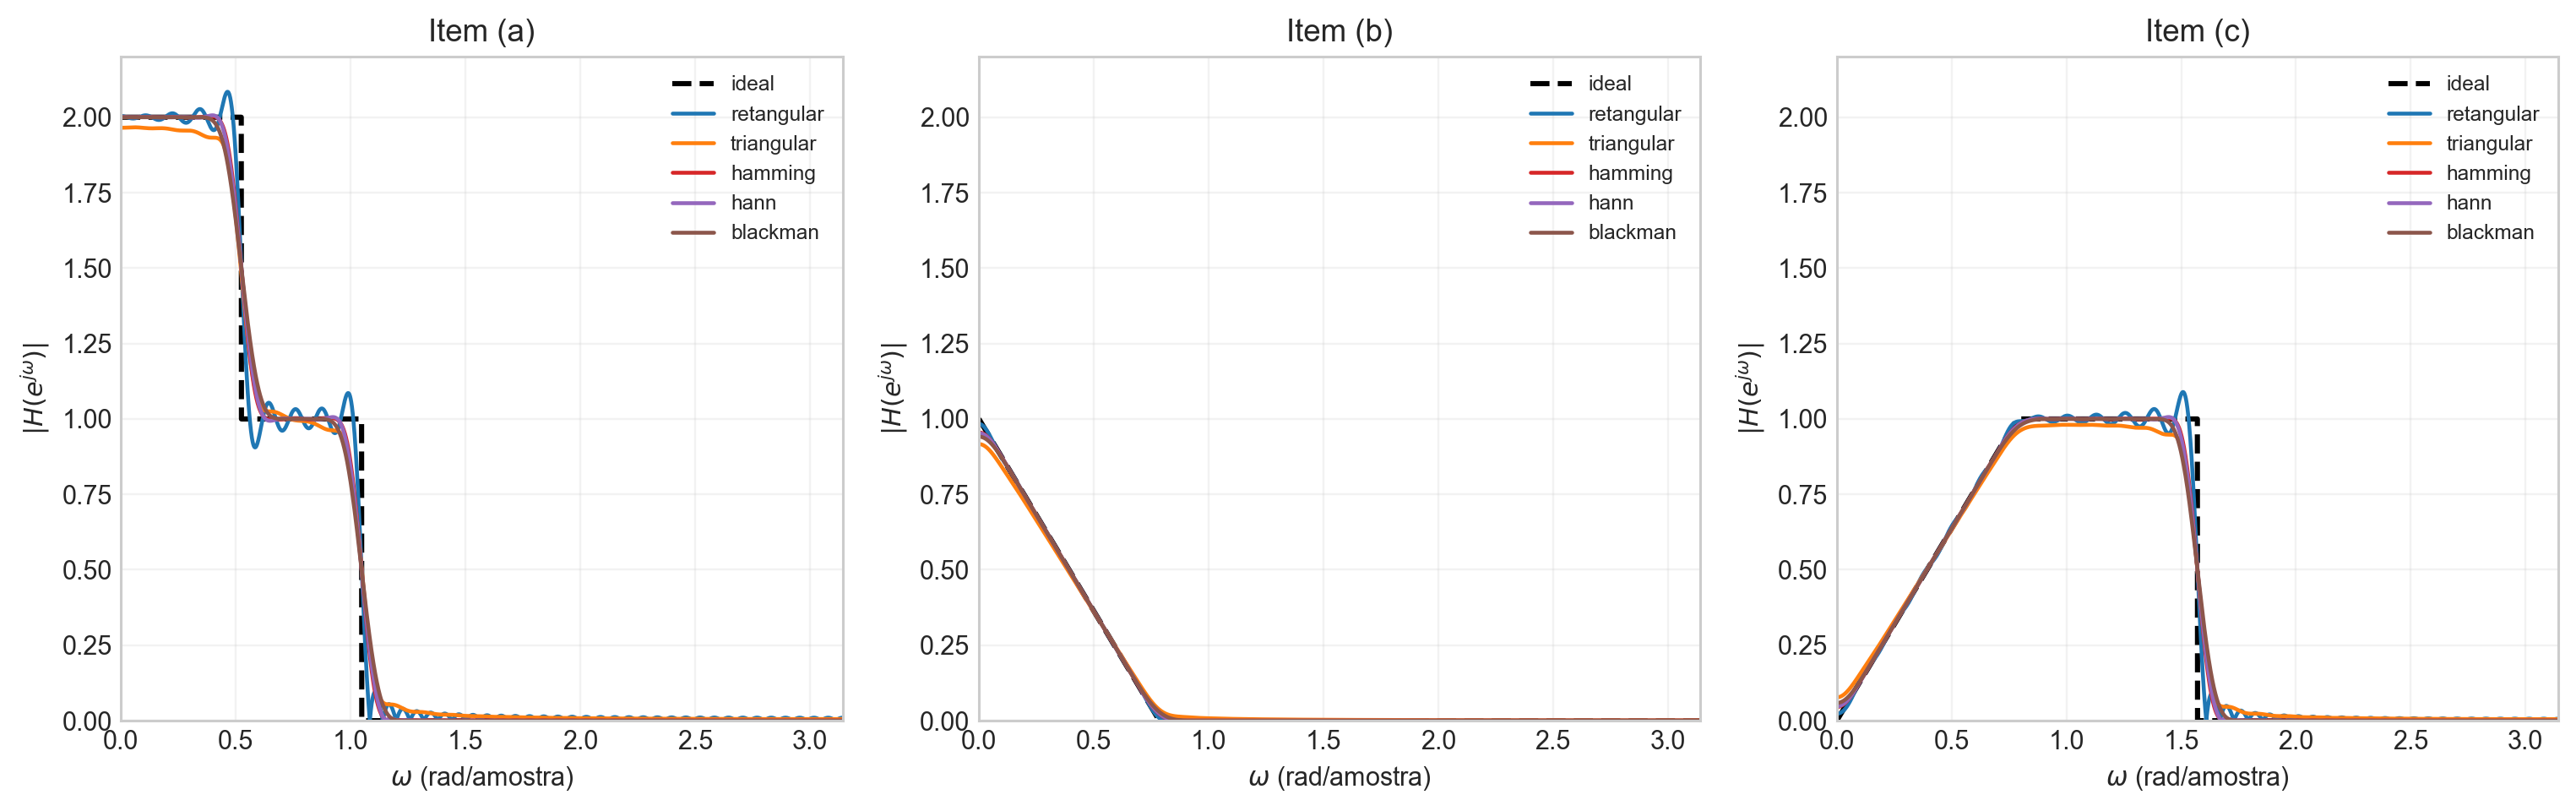
\includegraphics[width=\textwidth]{q2_responses_m100.png}
    \caption{Respostas em frequência da Questão 2 para $M=100$, com sobreposição da resposta ideal.}
    \label{fig:q2-respostas}
\end{figure}

\begin{table}[H]
    \centering
    \caption{Melhor janela por erro RMS nas ordens pedidas para a Questão 2.}
    \begin{tabular}{lcccc}
\toprule
Caso & Melhor janela, $M=50$ & Erro RMS & Melhor janela, $M=100$ & Erro RMS \\
\midrule
Item (a) & retangular & 0,0889 & retangular & 0,0619 \\
Item (b) & retangular & 0,0034 & retangular & 0,0012 \\
Item (c) & retangular & 0,0626 & retangular & 0,0451 \\
\bottomrule
\end{tabular}
\end{table}

O item (b) foi o mais fácil de aproximar numericamente, pois sua resposta ideal já é suave e limitada a uma região estreita de baixas frequências. Por isso, os erros RMS ficaram muito menores do que nos itens (a) e (c). Novamente, o aumento de ordem melhorou a aproximação em todos os casos.

Entretanto, o mesmo cuidado observado na Questão 1 vale aqui: o erro RMS global tende a favorecer respostas mais ``agressivas'' em transição, especialmente a janela retangular. Isso não significa melhor comportamento visual em banda de rejeição. Nas figuras, Hamming, Hann e Blackman apresentam menos ondulações, o que torna essas janelas mais atraentes quando a prioridade é suavidade espectral.

\section*{Questão 3: Filtragem do Áudio Contaminado}
Na última questão, o objetivo foi recuperar o sinal \texttt{handel.wav} contaminado por um tom de 100 Hz, um tom de 2000 Hz e ruído branco com variância $\sigma^2 \in \{10^{-2}, 10^{-1}, 1\}$. A escolha do sistema FIR foi guiada pela comparação com a Prática 6: o passa-altas em 180 Hz foi mantido para remover a componente de baixa frequência, mas o simples passa-baixas em 1800 Hz foi substituído por uma rejeição estreita em torno de 2000 Hz, preservando melhor o restante da banda útil.

\begin{figure}[H]
    \centering
    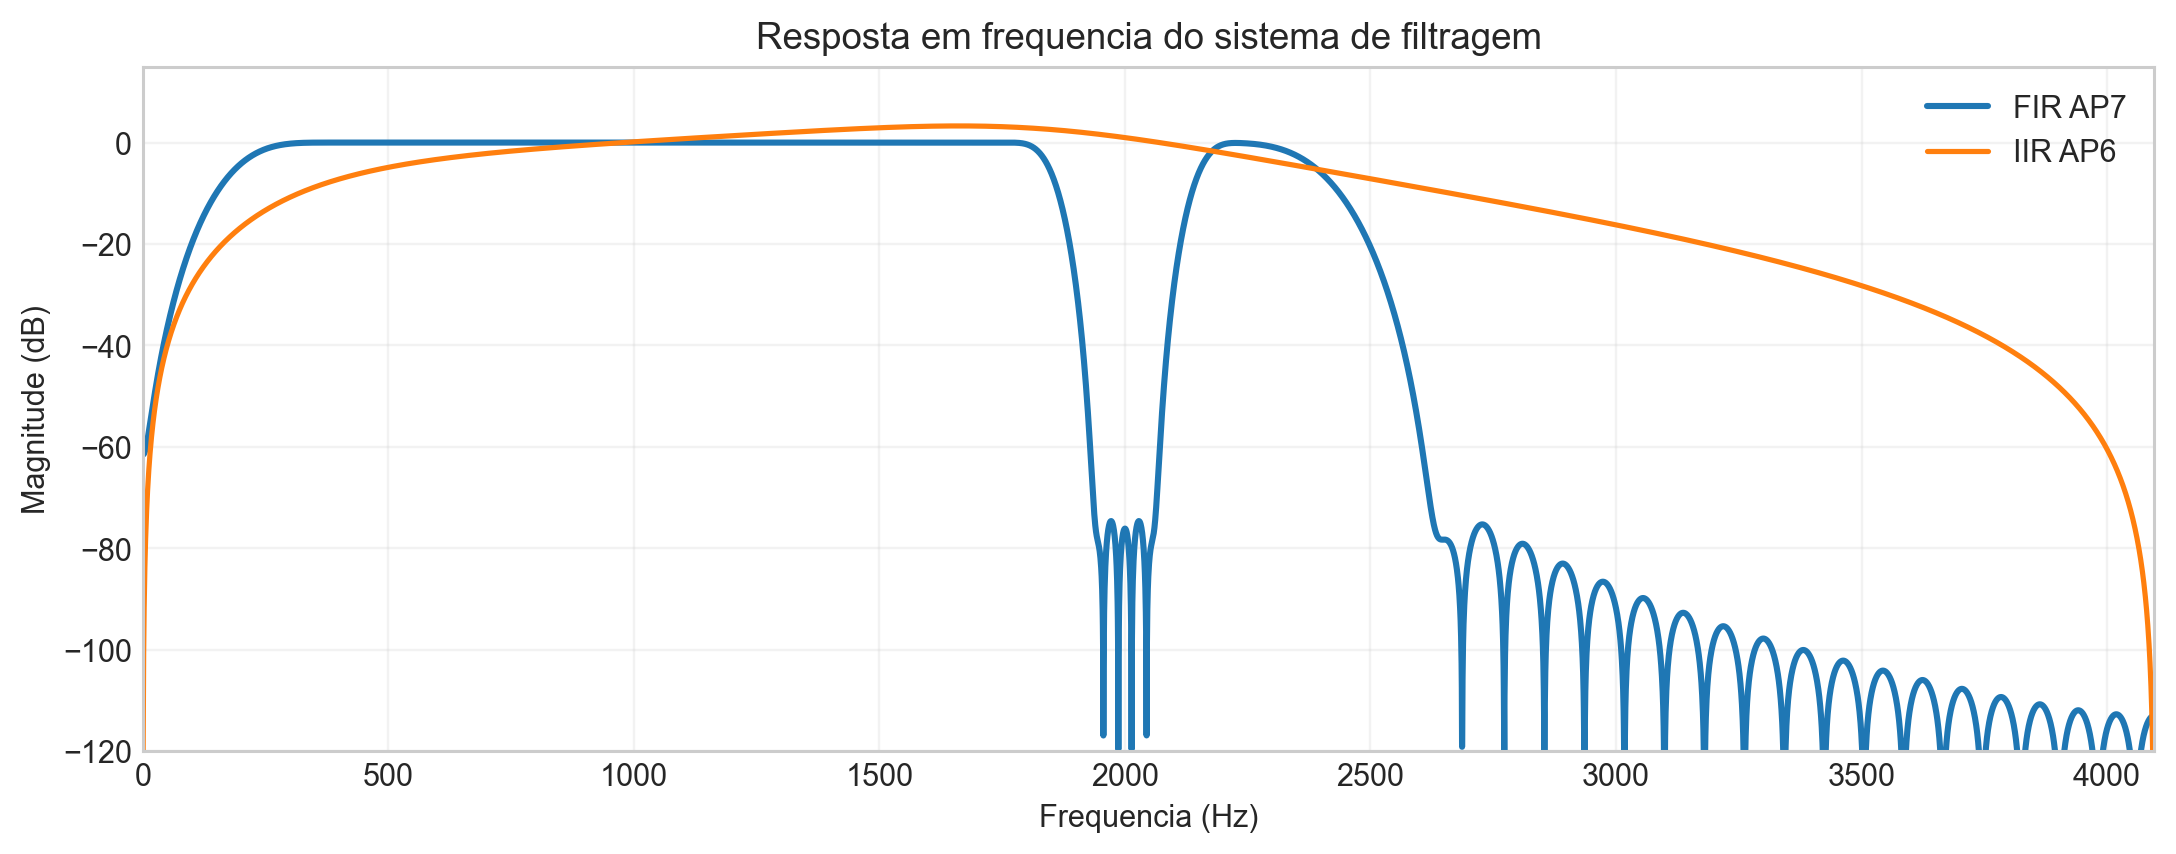
\includegraphics[width=0.95\textwidth]{q3_system_response.png}
    \caption{Resposta em frequência do sistema FIR da Prática 7 e comparação com a referência IIR da Prática 6.}
    \label{fig:q3-resposta}
\end{figure}

\begin{figure}[H]
    \centering
    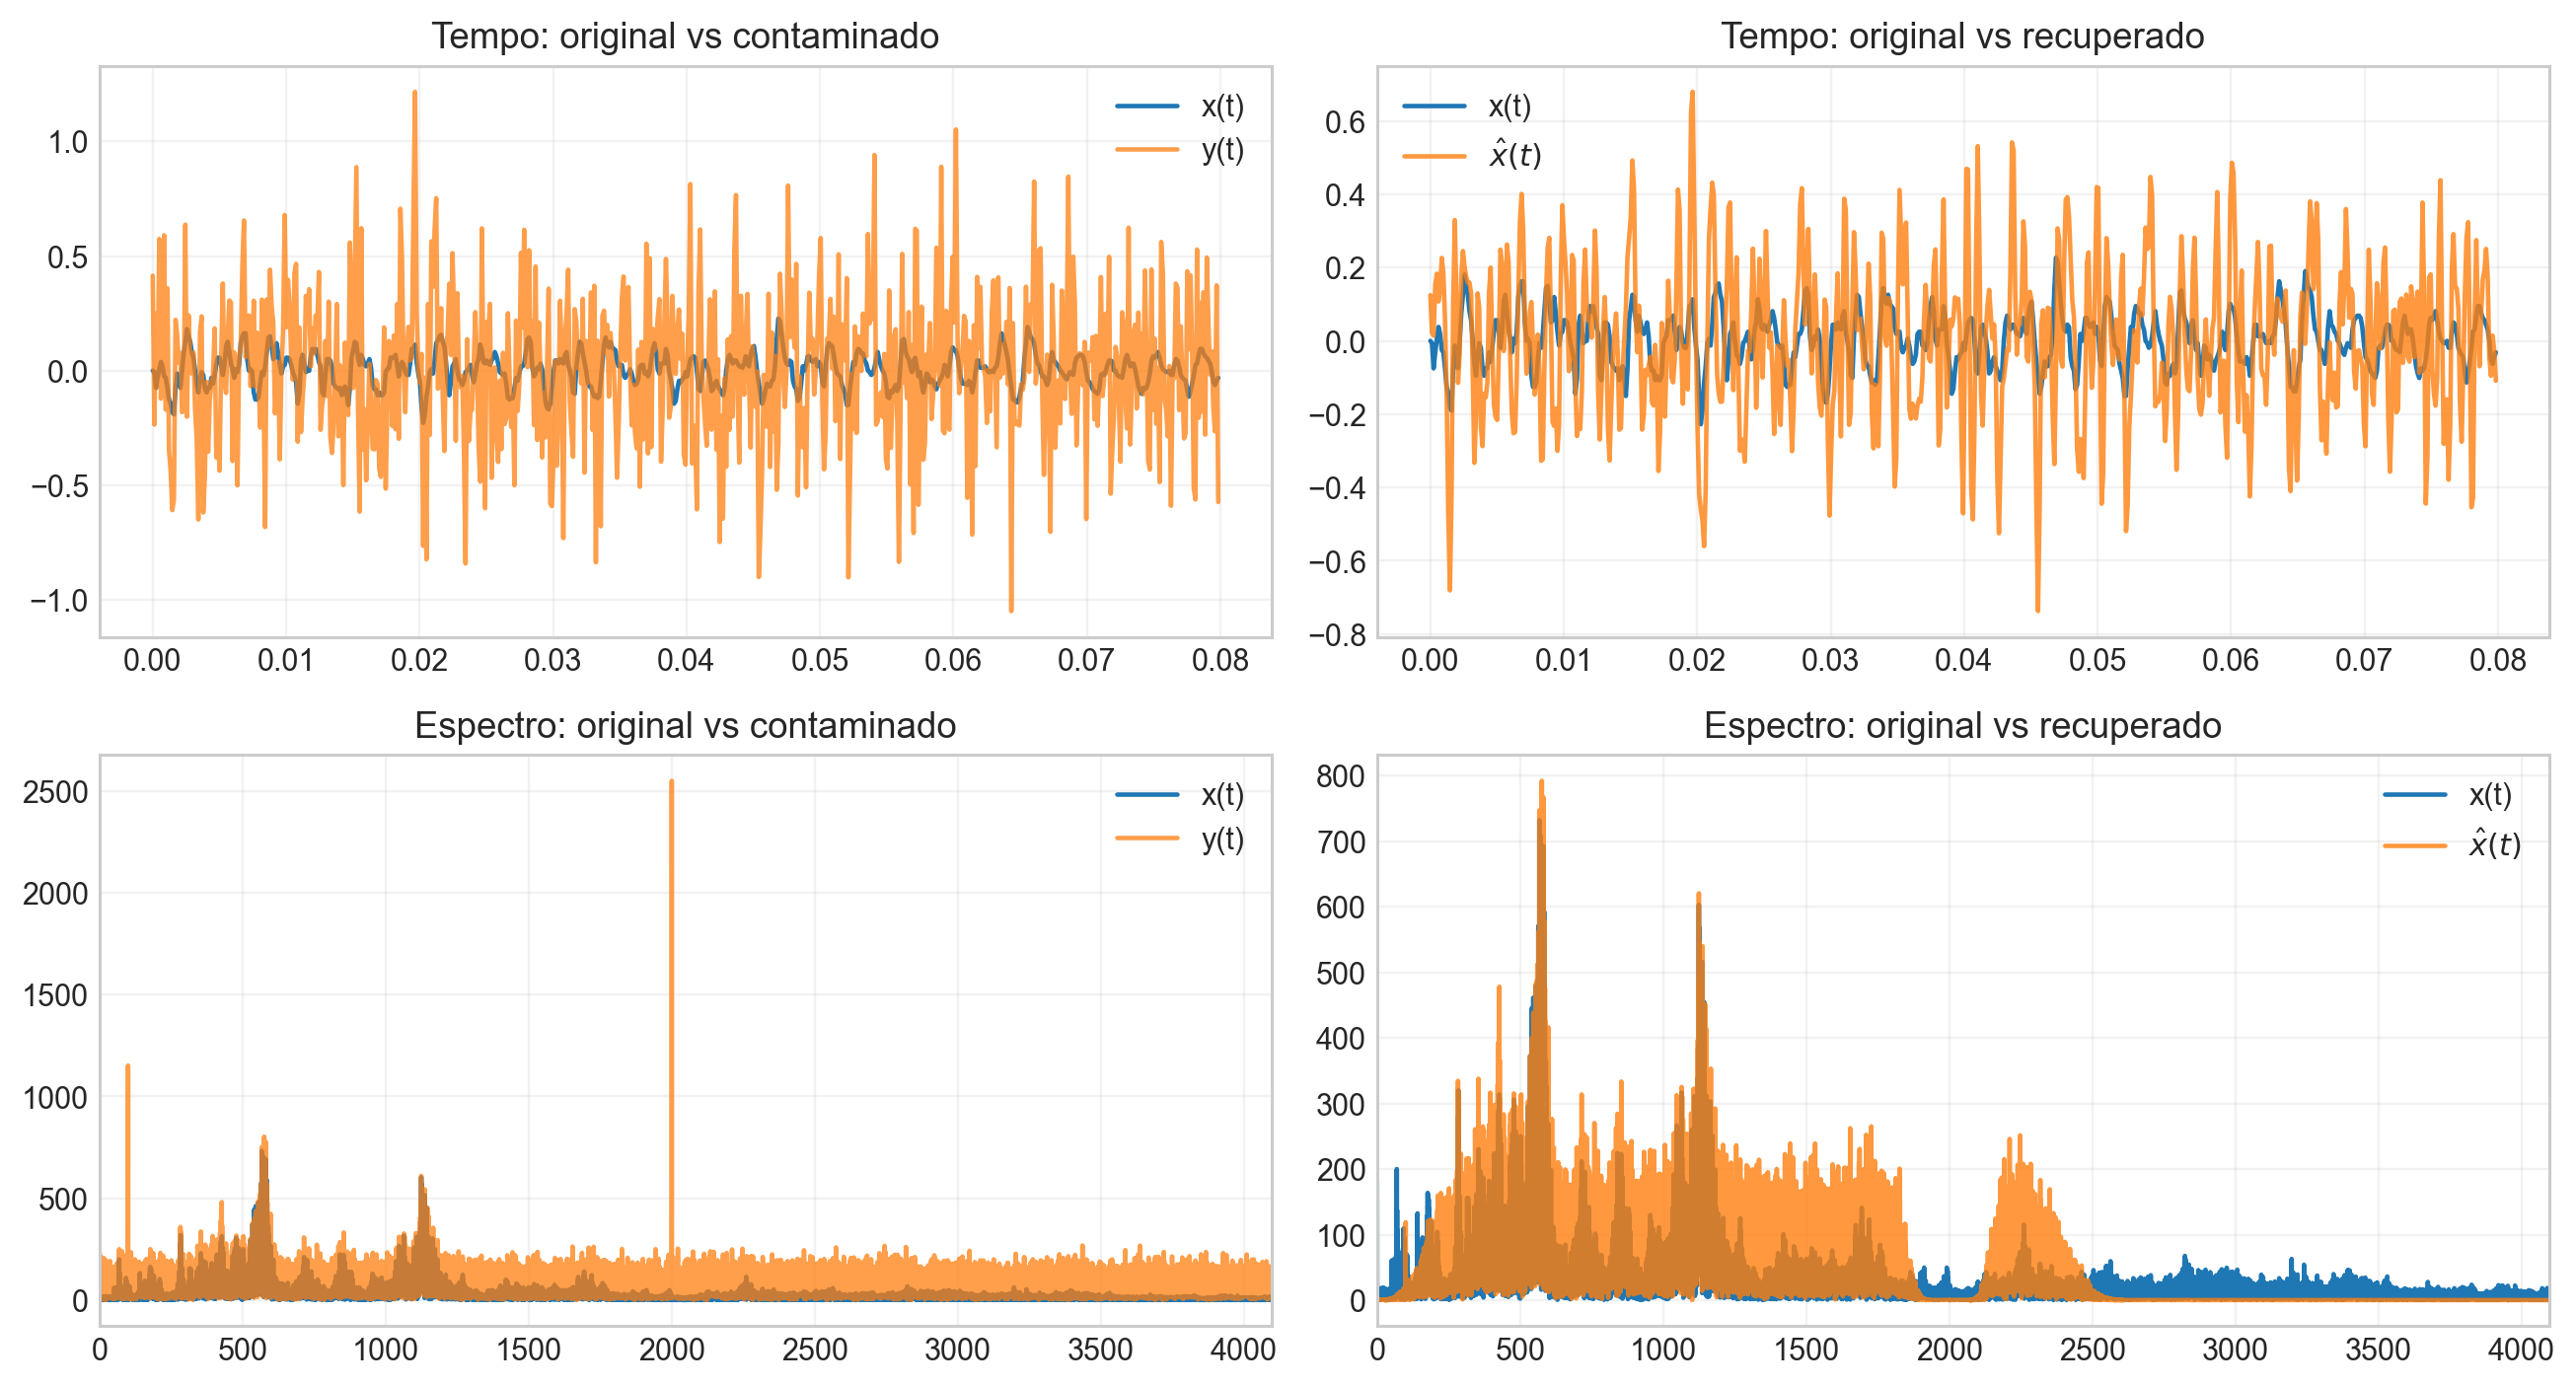
\includegraphics[width=\textwidth]{q3_compare_sigma_0_1.png}
    \caption{Comparação entre áudio original, contaminado e recuperado pelo sistema FIR para $\sigma^2 = 10^{-1}$.}
    \label{fig:q3-audio}
\end{figure}

\begin{table}[H]
    \centering
    \caption{Comparação quantitativa entre o sistema FIR da Prática 7 e a referência IIR da Prática 6.}
    \resizebox{\textwidth}{!}{\begin{tabular}{lcccccc}
\toprule
$\sigma^2$ & SNR entrada (dB) & FIR SNR (dB) & FIR MSE & FIR pot. residual & IIR SNR (dB) & IIR MSE \\
\midrule
0,01 & 4,3934 & 8,0783 & 0,0060 & 0,0060 & 0,0525 & 0,0380 \\
0,1 & -4,2760 & -0,7332 & 0,0457 & 0,0457 & -3,6927 & 0,0901 \\
1 & -14,1724 & -10,6036 & 0,4433 & 0,4433 & -12,0631 & 0,6192 \\
\bottomrule
\end{tabular}}
    \end{table}

Os resultados indicam que o sistema FIR superou a referência IIR nos três cenários testados. Para $\sigma^2 = 10^{-2}$, a SNR de saída subiu de 0,05 dB para 8,08 dB. Em $\sigma^2 = 10^{-1}$, a SNR melhorou de -3,69 dB para -0,73 dB, com queda correspondente no MSE. Mesmo em $\sigma^2 = 1$, quando o ruído branco domina boa parte do espectro, o FIR ainda preservou vantagem em relação à solução da prática anterior.

Essa melhora acontece porque o novo sistema separa as tarefas. O passa-altas remove a interferência de 100 Hz, o rejeita-faixas ataca especificamente a região em torno de 2000 Hz e o passa-baixas reduz ruído acima de 2400 Hz sem cortar desnecessariamente toda a banda acima de 1800 Hz. Em consequência, o áudio recuperado tende a soar menos abafado do que na estratégia IIR usada na Prática 6.

\subsection*{Quantização dos Coeficientes}
Como o sistema permanece FIR após a quantização, a estabilidade não muda: os polos continuam na origem. O efeito dominante da quantização aparece, portanto, no deslocamento dos zeros e na alteração da resposta em frequência.

\begin{figure}[H]
    \centering
    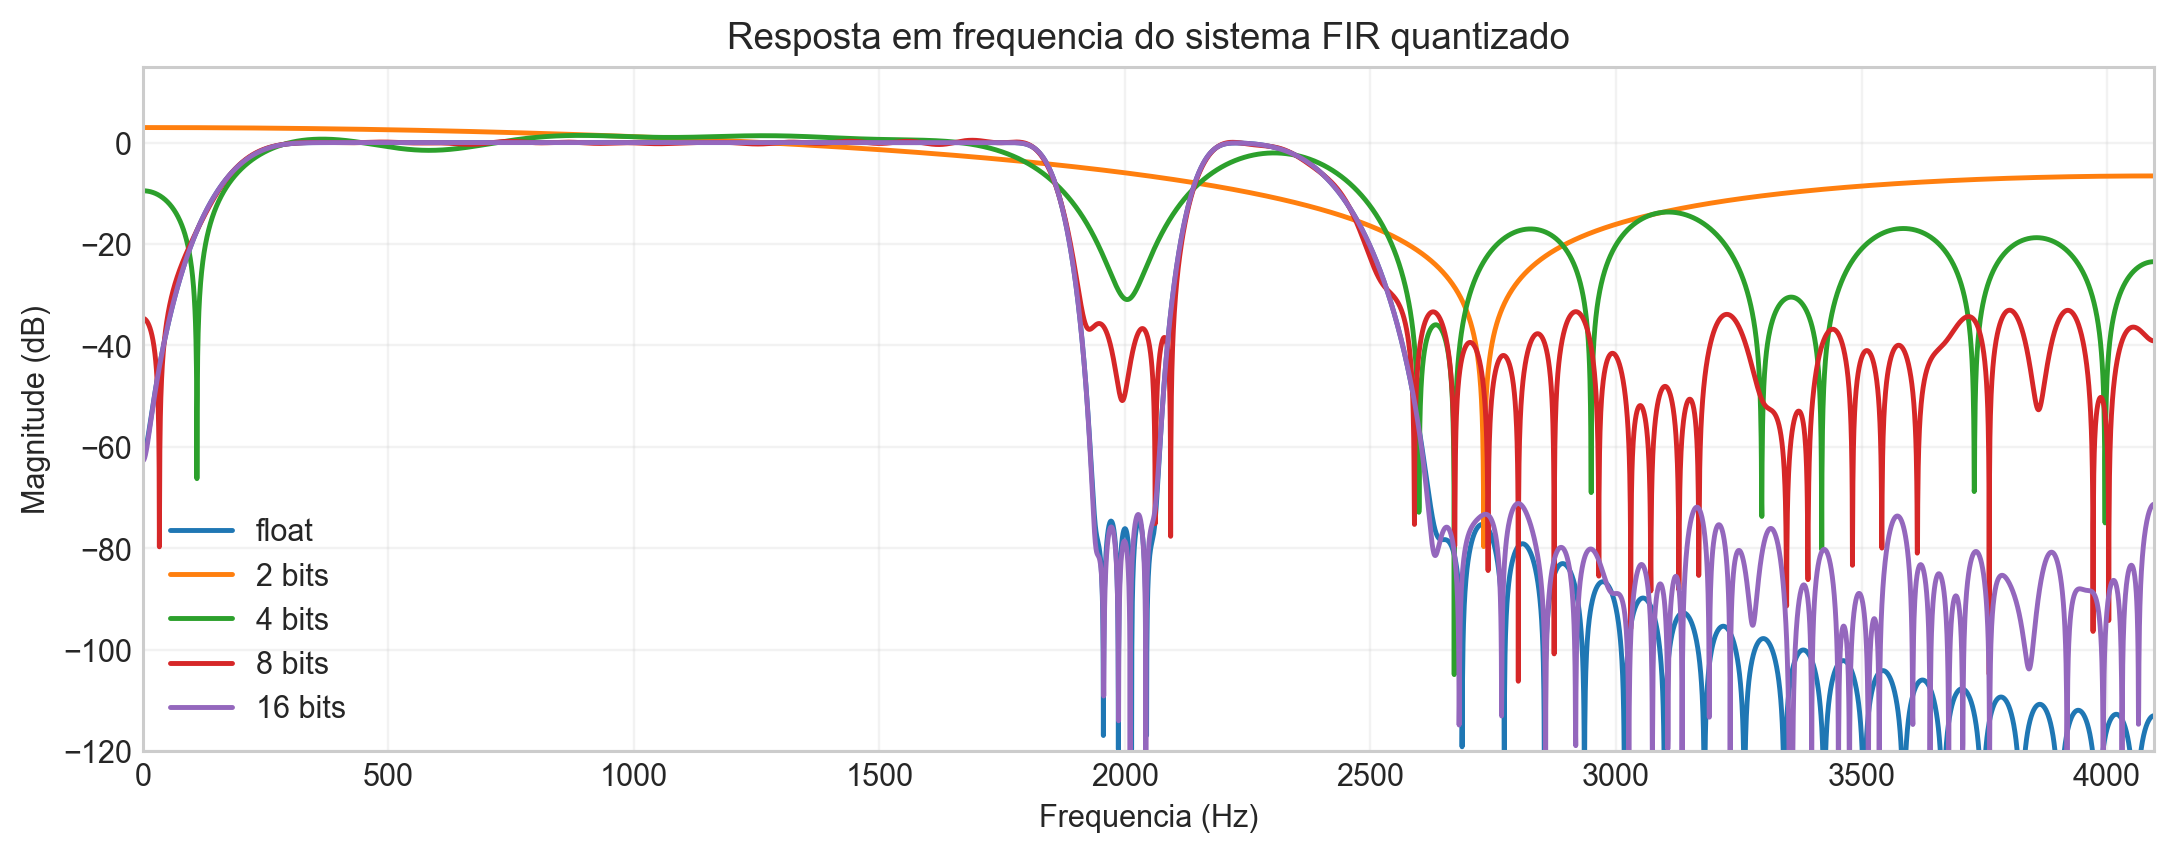
\includegraphics[width=0.95\textwidth]{q3_quantized_response.png}
    \caption{Resposta em frequência do sistema FIR original e quantizado.}
    \label{fig:q3-quant}
\end{figure}

\begin{table}[H]
    \centering
    \caption{Impacto da quantização no sistema FIR para $\sigma^2 = 10^{-1}$.}
    \begin{tabular}{lcccc}
\toprule
Filtro & SNR saida (dB) & MSE & Pot. residual & Coef. nao nulos \\
\midrule
float & -0,7332 & 0,0457 & 0,0457 & 481 \\
2 bits & -2,7727 & 0,0730 & 0,0730 & 3 \\
4 bits & -1,0573 & 0,0492 & 0,0492 & 21 \\
8 bits & -0,7215 & 0,0455 & 0,0455 & 97 \\
16 bits & -0,7331 & 0,0457 & 0,0457 & 241 \\
\bottomrule
\end{tabular}
\end{table}

O caso de 2 bits praticamente descaracteriza o filtro, restando apenas três coeficientes não nulos. Em 4 bits, a estrutura básica já reaparece, mas o desempenho ainda fica bem abaixo da solução em ponto flutuante. A partir de 8 bits, as métricas ficam muito próximas do filtro original, e em 16 bits a diferença já é desprezível na prática.

Subjetivamente, o áudio recuperado com 8 e 16 bits mantém inteligibilidade próxima à versão em ponto flutuante, enquanto 2 e 4 bits introduzem distorções mais evidentes e rejeição menos controlada do tom em torno de 2000 Hz.

\section*{Resultados e Discussão}
A Prática 7 mostrou de forma clara o compromisso clássico dos filtros FIR por janelamento. Ordens maiores aproximam melhor a resposta ideal, mas aumentam custo computacional e atraso de grupo. Janelas suaves, como Hann, Hamming e Blackman, reduzem os ripples e melhoram a rejeição fora da banda, porém alargam a transição. Já a janela retangular oferece aproximação RMS global menor em alguns casos, mas com pior comportamento visual fora da banda desejada.

Em comparação com a Prática 6, a solução FIR se mostrou mais conveniente para o problema de áudio quando o objetivo é remover tons isolados sem sacrificar tanto a faixa útil. O preço pago foi um atraso fixo de aproximadamente 29,3 ms e um número maior de coeficientes. Ainda assim, a linearidade de fase e a seletividade do rejeita-faixas tornaram o resultado mais equilibrado do que a cascata IIR simples usada anteriormente.

\section*{Conclusão}
A Prática 7 consolidou o uso de respostas ideais e janelas como estratégia de projeto FIR. O método permite controlar explicitamente a forma espectral do filtro, garante estabilidade por construção e facilita a obtenção de fase linear, o que foi especialmente útil na aplicação com áudio.

Os resultados confirmaram que a ordem do filtro e a escolha da janela influenciam diretamente o compromisso entre seletividade e suavidade espectral. Na aplicação prática, a combinação passa-altas + rejeita-faixas + passa-baixas superou a referência IIR da Prática 6 para todos os níveis de ruído testados. A quantização mostrou que 8 bits já oferecem desempenho próximo ao caso em ponto flutuante, enquanto quantizações muito agressivas degradam fortemente a filtragem.

\section*{Referências}
CHAVES, Rafael. \textbf{Aula Prática 7: Projeto de Filtros FIR}. Processamento de Sinais I.

OPPENHEIM, Alan V.; SCHAFER, Ronald W. \textbf{Discrete-Time Signal Processing}. 3. ed. Upper Saddle River: Pearson, 2010.

PROAKIS, John G.; MANOLAKIS, Dimitris G. \textbf{Digital Signal Processing: Principles, Algorithms, and Applications}. 4. ed. Pearson, 2007.

Documentação oficial do SciPy Signal: \url{https://docs.scipy.org/doc/scipy/reference/signal.html}.

\end{document}
